\documentclass[lang=cn, 11pt,   a4paper]{elegantpaper}

\usepackage{ctex}
\usepackage{amsfonts}
\usepackage{amsmath}
\usepackage{mathrsfs}
\usepackage[linesnumbered, ruled]{algorithm2e}
\usepackage{hyperref}
\usepackage{algorithmic}
\usepackage{listings}
\usepackage{color}
\usepackage{graphicx}
\usepackage{float}

\newcommand{\mb}{\mathbf}

\title{概率论研讨课期末实践作业\\ CIFAR-100图像数据集的分类问题 -- 思考与讨论}
\author{韩菲雨, 林津伊, 孙睿, 孙行之, 谢沁昕, 应东昊\\中国科学院大学}

\date{\today}

\begin{document}

\maketitle

\begin{abstract}
图像分类在近若干年一直是计算机视觉研究的热点问题. 本文介绍了本组为实现CIRFAR-100图像数据集的分类问题所进行的调研过程, 及最终采取的方案. 在调研过程中, 我们考察了朴素贝叶斯, K-近邻等多种方法, 最后我们决定采用卷积神经网络模型. 在提供基础的解决方案之外, 我们还参考前人的工作, 给出了适应于该问题的改进方案 -- 层级深度卷积神经网络模型
\end{abstract}

\keywords{} 图像分类, 卷积神经网络


\tableofcontents

\section{引言}
目前,主流的图像分类技术可划分为基于传统机器学习的方法以及基于深层网络模型的深度学习方法. 传统机器学习方法基本的思路是首先对预处理完后的数据进行特征提取;紧接着,分类器基于提取后的特征进行训练. 由于手工提取特征方法和分类器都是基于一定的理论基础进行设计,因此具有较好的可解释性. 

然而,传统机器学习方法的效果过度依赖于特征,而手工设计的特征具有较大的局限性且难于设计,因此仍无法胜任一些复杂的任务. 深度学习算法通过深层的网络结构将特征提取任务和分类器以端到端的方式整合到同一个网络中,并使用大量的标注样本通过反向传播机制不断更新模型参数,从而同时提升模型的特征提取和分类的能力. 

我们组前期对多种传统的机器学习方法进行调研,包括朴素贝叶斯方法, BP神经网络方法, 迁移模型方法, CNN方法, K-近邻方法, 支持向量机方法等. 最后综合比较下,我们决定通过卷积神经网络 (CCN) 实现图像分类. 在代码实现方面, 我们给出了K-近邻方法与CNN方法的完整代码. 此外, 我们借鉴前人的工作, 给出了一种改进方法 (HD-CNN) 的代码实现. 但因空间与时间的限制, 我们建立的CNN模型与HD-CNN模型没有运行出完整的结果 (代码预期运行时间分别为17小时与21小时). 代码与运行结果整理参见: \href{https://github.com/dalek-supreme/CIFAR-100-classification-with-CNN}{https://github.com/dalek-supreme/CIFAR-100-classification-with-CNN}

\section{研讨过程}
\subsection{朴素贝叶斯}
朴素贝叶斯是一种极其简单的分类算法,通过概率统计到的方式进行判别. 通过特征的联合概率分布$P\left (w_{1}, w_{2}, w_{3}, \cdots w_{n} | C\right)$建模,进而利用贝叶斯公式得到$P\left (C | w_{1}, w_{2}, w_{3}, \cdots w_{n}\right)$. 目标是根据特征得到属于某一类的概率,哪一类的概率最大则是哪一类. $P (C)$根据大数定律,我们通过频率来代替概率. 建模关键点还是在于$P (w|C)$的求解,$w$为特征向量,则
\begin{equation}
P (w | C)=P\left (w_{1}, w_{2}, w_{3}, \cdots w_{n} | C\right)
\end{equation}

我们假设这些特征是线性无关的,则可得$P (w | C)=P\left (w_{1} | C\right) P\left (w_{2} | C\right) P\left (w_{3} | C\right) \cdots P\left (w_{n} | C\right)$, 即我们需要求解在某类条件下某一个特征的概率. 

利用训练集创建好词袋模型后,即可得到每个特征在对应条件下的概率,即建立好模型. 将测试集图像样本转换为向量模型后导入创建好的模型,得到预测结果. 我们测试发现在数据集数量小的情况下能达到不错的效果,但是基于朴素贝叶斯对图像进行分类往往就很难用尝试去理解其中的原因. 因为它的特征我们假设都是线性无关的,对于图像来说这往往不科学,相邻两个像素值往往关系更大. 

不仅如此,对于$P (w | C)=P\left (w_{1} | C\right) P\left (w_{2} | C\right) P\left (w_{3} | C\right) \cdots P\left (w_{n} | C\right)$满足乘法交换法则,也就是说像素的随机组合导致图像可能变的很糟糕,但是他们的效果确是相同的. 

\subsection{迁移模型}
迁移学习可以利用其他模型在学习其他模型已经训练得到的模式和知识,并应用到当前你要解决的问题中. 进行迁移学习之前,我们需要和我们解决问题不一样的预训练模型. 对于图像分类的迁移学习任务,我们无法使用自然语言处理的预训练模型,通常情况下,我们会选择一些训练目标类似的预训练模型用于迁移学习. 

实际操作中,我们首先将数据和任务分成四类
\begin{enumerate}
\item 大数据集+与预训练目标有较大不同;
\item 大数据集+与预训练目标相似;
\item 小数据集+与预训练目标有较大不同;
\item 小数据集+与预训练目标相似. 
\end{enumerate}

我们用的数据集,每个类别只有600个图像 (小于1000),按照经验,划分为小数据集. 

第二步,制定与上述四类对应的微调策略. 在我们的情况中,我们分两种情况. 处于第三类时: 数据集较小,并且与预训练模型的目标不同. 这是最糟糕的情况了,由于数据集太小我们不能全量训练,又由于训练目标不同我们不得不尽可能多的训练中间层. 处于第四类时: 小数据集,但与预训练模型的目标类似. 这种情况下,你只需要重新训练分类器即可,避免过拟合的同时又能确保你的目标得到了训练. 

由于无法找到预训练的对象,以及考虑到迁移学习的过适配问题. 我们暂且对此方法保留,后续可以考虑利用迁移学习对CNN的优化. 

\subsection{支持向量机}
支持向量机 (Support vector machines,  SVM)是一种二分类模型, 它的基本模型是定义在特征空间上的间隔最大的线性分类器. 支持向量机的学习策略是间隔最大化, 可形式化为一个求解凸二次规划的问题, 其算法就是求解凸二次规划的最优算法. 

\subsubsection{支持向量机模型的原问题与对偶问题}
给定训练集$D=\left\{\left (x_{1},  y_{1}\right), \left (x_{1},  y_{1}\right) \ldots \ldots\left (x_{m},  y_{m}\right)\right\},  y_{i} \in\{1, -1\}$,  分类学习的思想就是基于训练集D在样本空间中找到一个超平面:  $w^{T} x+b=0$ 将不同类别的样本分开,  其中$w = (w_1,  w_2,  \dots,  w_d)$为法向量.

考虑到训练集的局限性和噪声等因素, 应使两侧样本尽可能离超平面较远, 保证超平面受影响小, 这样的分类结果才更具有鲁棒性. 假设超平面能将样本正确分类:  当$y_1 = +1$时,  称为正例,  有$w^Tx_i +b \ge 1$; 当$y_1 = -1$时,  称为负例,  有$w^Tx_i +b \le -1$. 使得距离超平面最近的训练样例使上式的等号成立, 它们被称为支持向量. 两个分类到超平面距离之和为 $\gamma=\frac{2}{\|\mathrm{w}\|}$,  称为间隔. 

欲找到间隔最大的划分超平面, 即找到$w$和$b$使得 $\gamma$ 最大: 
\begin{equation}
\label{svm primal}
\begin{array}{c}
{\max _{w,  b} \frac{2}{\|w\|}} \\
{\text {subject to } y_{i}\left (w^{T} x_{i}+b\right) \geq 1}
\end{array}
\end{equation}

显然, 最大化间隔即为最小化$\|w\|$,  这即是支持向量机的基本模型. 我们可用拉格朗日乘子法得到其该问题的对偶问题. 将问题\ref{svm primal}写成最小化的形式后,  其对应的拉格朗日函数是
\begin{equation}
L (w,  b,  \alpha)=\frac{1}{2}\|w\|^{2}+\sum_{i=1}^{m} \alpha_{i}\left (1-y_{i}\left (w^{T} x_{i}+b\right)\right)
\end{equation}

考虑拉格朗日函数关于变量$w, b$的极小值,  对应偏导为0,  即成立
\begin{equation}
w=\sum_{i=1}^{m} \alpha_{i} y_{i} x_{i} \quad 0=\sum_{i=1}^{m} \alpha_{i} y_{i}
\end{equation}

从而可以将原问题转化为关于$\alpha$的对偶问题
\begin{equation}
\begin{array}{c}
{\max _{\alpha} \sum_{i=1}^{m} \alpha_{i}-\frac{1}{2} \sum_{i}^{m} \sum_{j=1}^{m} \alpha_{i} \alpha_{j} y_{i} y_{j} x_{i}^{T} x_{j}}\\
{\text{s.t.} \alpha \geq 0,  \sum_{i=1}^{m} \alpha_{i} \cdot y_{i}=0}
\end{array}
\end{equation}

通过求解该问题,  我们可以得到最终的模型$f (x)=\sum_{i=1}^{m} \alpha_{i} y_{i} x_{i}^{T} x+b$,  其中解应当满足约束优化的KKT的条件
\begin{equation}
\left\{\begin{array}{rl}
{\alpha_{i} \geq 0} \\
{y_{i} f (x)-1 \geq 0} \\
{\alpha_{i}\left (y_{i} f (x)-1\right)=0}
\end{array} \right.
\end{equation}
求解该问题的优化方法有很多,  常用的方法例如Sequential Minimal Optimization,  SMO.

\subsubsection{线性支持向量机与软间隔化}
硬间隔的分类法其结果容易受少数点的控制, 这是很危险的. 这里给出的解决方法是: 允许一些点到分类平面的距离不满足原先的要求. 由于不同的训练集各点的间距尺度不太一样, 因此用间隔来衡量有利于我们表达形式的简洁. 我们原先对样本点的要求是 $y_{i}\left (w^{T} x_{i}+b\right) \geq 1$. 现在对每个点引入一个松弛变量$\xi_i\ge 0$, 则约束条件变为: 
\begin{equation}
y_{i}\left (w^{T} x_{i}+b\right) \geq 1-\xi_{i}	
\end{equation}
则原来的目标函数变为
$\min _{w,  b} \frac{1}{2}\|w\|^{2}+C \sum_{i=1}^{N} \xi_{i}$
同理求解拉格朗日函数可得到相应的对偶问题. 当然线性支持向量机学习还有另一种解释, 就是最小化目标函数
\begin{equation}
\sum_{i=1}^{N}\left[1-y_{i}\left (w^{T} x_{i}+b\right)\right]_{+}+\lambda\|w\|^{2}
\end{equation}

其中$\left[1-y_{i}\left (w^{T} x_{i}+b\right)\right]_{+}$被称为合页损失函数. 

\subsubsection{核函数}
在处理线性不可分的问题时通常将数据从一个特征空间转换到另一个特征空间, 在新的特征空间下往往有比较清晰的测试结果. 如果原始空间是有限维的, 即属性有限, 则一定存在一个高维特征空间使样本可分. SVM中优化目标函数是写成内积的形式, 我们假设$\phi (x)$表示将$x$映射后的特征向量, 那么优化目标函数变成: 
\begin{equation}
\max _{\alpha} \sum_{i=1}^{m} \alpha_{i}-\frac{1}{2} \sum_{i=1}^{m} \sum_{j=1}^{m} \alpha_{i} \alpha_{j} y_{i} y_{j} \phi\left (x_{i}\right)^{T} \phi\left (x_{j}\right)
\end{equation}
要想直接求解$\phi\left (x_{i}\right)^{T} \phi\left (x_{j}\right)$是困难的. 为了避开这个障碍, 就设想了一个函数$$k\left (x_{i},  x_{j}\right)=\phi\left (x_{i}\right)^{T} \phi\left (x_{j}\right)$$

\subsubsection{实现思路}
导入数据进行预处理, 计算SVM的合页损失函数和梯度, 选择$w$使得损失函数最小进行优化 (具体通过梯度来实现), 并对数据进行训练与预测. 


\section{神经网络}
神经网络是最著名的机器学习模型之一, 是人们受到构成动物大脑的生物神经网络的启发而构建的特殊的计算系统. 生物神经系统主要由神经元和网络结构组成, 网络结构将不同的神经元连接起来形成一个巨大的网络. 神经元可以通过树突从其他细胞接收信息, 同时使用轴突将消息传递到其他的神经元. 受此启发, 研究人员使用类似的概念构建了人工神经网络 \cite{周16}. 
\subsection{神经元与前馈神经网络}

正如神经元是构成生物神经网络的最基本的单元, 人工神经网络中也有\textit{神经元}的概念.
\begin{figure}[h]
\centering{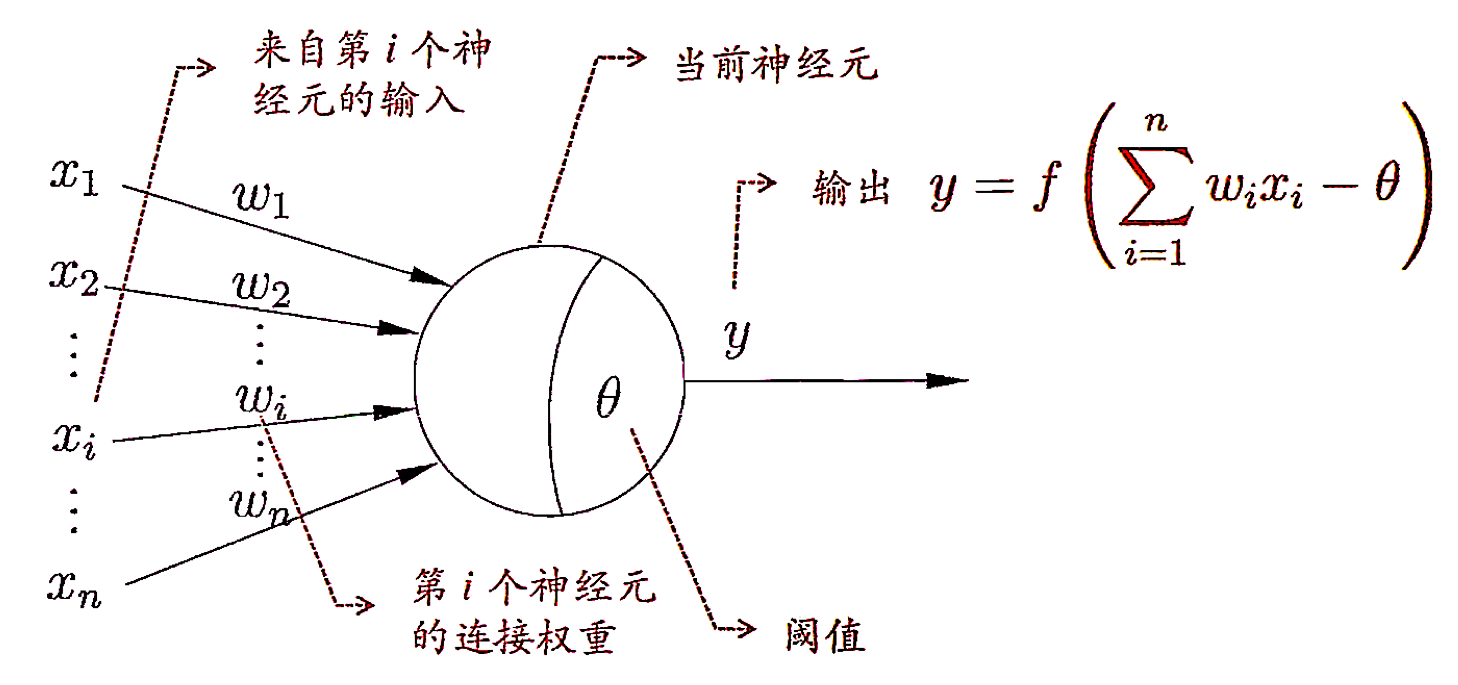
\includegraphics[height=4cm]{nervecell.png}}
\caption{神经元示意图}
\end{figure}

一个神经元接受其他神经元传递的信息作为输入. 在使用激活函数$y = f \left ( \sum _ { i = 1 } ^ { n } w _ { i } x _ { i } - \theta \right)$处理后, 该神经元将输出传递到之后的神经元. 在神经网络的训练中, 我们最终想要学习的参数即为激活函数中的系数$\omega_i, \theta$. 这里的另一个关键点是, 我们需要选择一个合适的函数作为神经元的激活函数. 我们希望该激活函数具有分类的能力, 例如, 将一组样本映射到1, 而将其他样本映射到0, 如下的阶梯函数是一个理想的例子:  
$$
{ f } ( x ) = \left\{ \begin{array} { l l } { 1, } & { x \geq 0 } \\ { 0, } & { x < 0 } \end{array} \right.
$$

但是, 该函数在$x=0$时存在突跃, 因而不可微, 这表明它不适用于梯度下降法. 我们更希望找到一个具有相似作用并且可微的激活函数. $Sigmoid$函数是一个不错的选择: 
\begin{equation}
 { sigmoid } ( x ) = \frac { 1 } { 1 + e ^ { - x } }
\end{equation}

通过示意图我们可以看到, $Sigmoid$函数以$y$轴作为分界线, 中心对称并且可微. 因此, 我们对于最后的输出, 我们也可以认为输出$=1$若$sigmoid (x) \ge 0$. 
\begin{figure}[H]
\centering{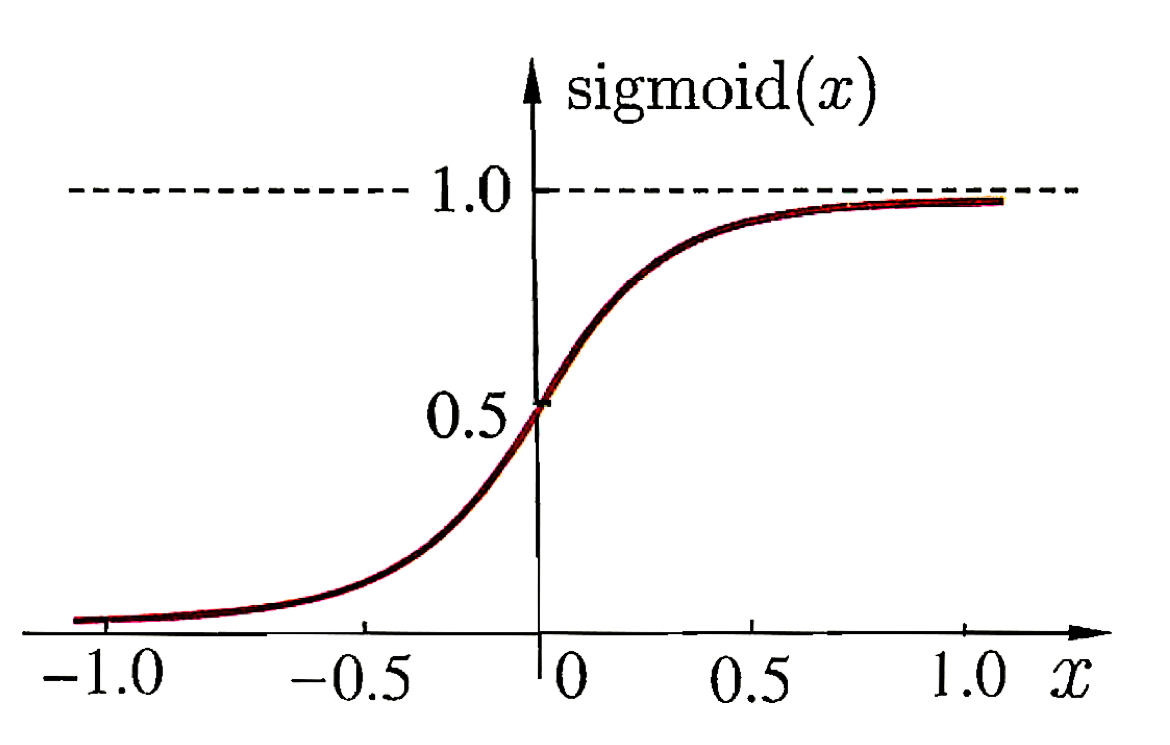
\includegraphics[height=4cm]{sigmoid.png}}
\caption{$Sigmoid$函数}
\end{figure}

神经元之间可以通过多种方式相互连接, 构建出不同的网络, 最常见的一种神经网络是多层前馈神经网络 (MFN), 在MFN中, 神经元按照层级排列, 每一层的神经元与其前后相邻层的神经元进行全连接, 信息单向传递. 一般认为, MFN的第一层和最后一层为输入和输出层, 输入和输出层之间的层称为隐藏层. 
\begin{figure}[h]
\label{fig: fullconnection}
\centering{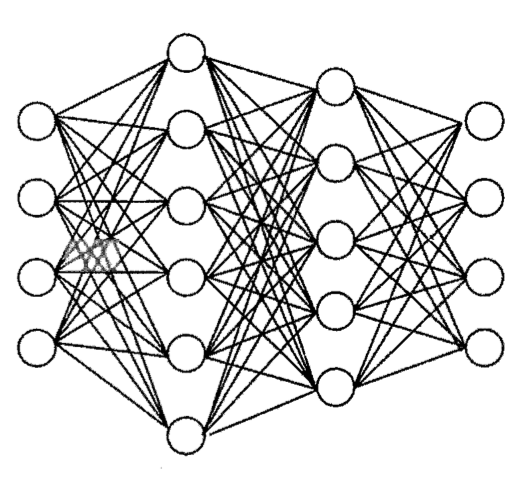
\includegraphics[height=5cm]{MFN.png}}
\caption{隐藏层数为2的前馈神经网络\cite{raschka15}}
\end{figure}

在神经网络的训练中, 通常会引入一个误差函数评判神经网络在训练样本上的表现, 例如$E_{k}=\frac{1}{2} \sum_{j=1}^{l}\left (\hat{y}_{j}^{k}-y_{j}^{k}\right)^{2}$, 其中$y_{j}^{k}$是样本真实标签值, $\hat{y}_{j}^{k}$是网络的预测值, 通常基于梯度下降法的反向传播算法 (Error Backpropagation Algorithm, BP算法) 是训练MFN最常用的算法之一, 以其表达的简单性与易理解性出名. BP 算法是一个迭代算法,它的基本思想为: (1) 先计算每一层的状态和激活值,直到最后一层;(2) 计算每一层的误差,误差的计算过程是从最后一层向前推进的,在反向传播中修改网络节点中的权重系数; (3) 更新参数使误差变小. 迭代前面两个步骤,直到满足停止准则,例如误差小于精度阈值. 我们请读者阅读\cite{周16, Mitchell97}以了解算法的详细推导过程及证明. 

神经网络已经被证明具有“解决”任意复杂度的问题的能力 (即具备全局近似的能力), 该结果具有多个版本, 以及多种证明的方式, 有兴趣的读者可以参照其中一个较为经典的结果\cite{hornik89}.

\subsection{卷积神经网络及其结构}
为了解决图像分类识别的问题,我们决定采取一种广泛应用于深度学习领域的神经网络,卷积神经网络.在本节中将简单介绍卷积神经网络的基本结构和性质.

深度学习的许多研究成果, 离不开对大脑认知原理的研究, 尤其是视觉原理的研究. 1981 年的诺贝尔医学奖, 颁发给了 David Hubel, TorstenWiesel, 以及 Roger Sperry. 前两位学者的主要贡献是\textit{发现了视觉系统的信息处理方式} -- 可视皮层是分级的.

人类的视觉原理如下:  从原始信号摄入开始, 瞳孔会摄入像; 接着做初步处理, 大脑皮层的某些细胞会发现图像中的边缘和方向的信息; 然后进行抽象, 例如大脑判定, 眼前的物体的形状是圆形的; 紧接着会进一步抽象, 例如进一步判定该物体是只气球. 下面是人脑进行人脸识别的一个示例:  
\begin{figure}[H]
\centering{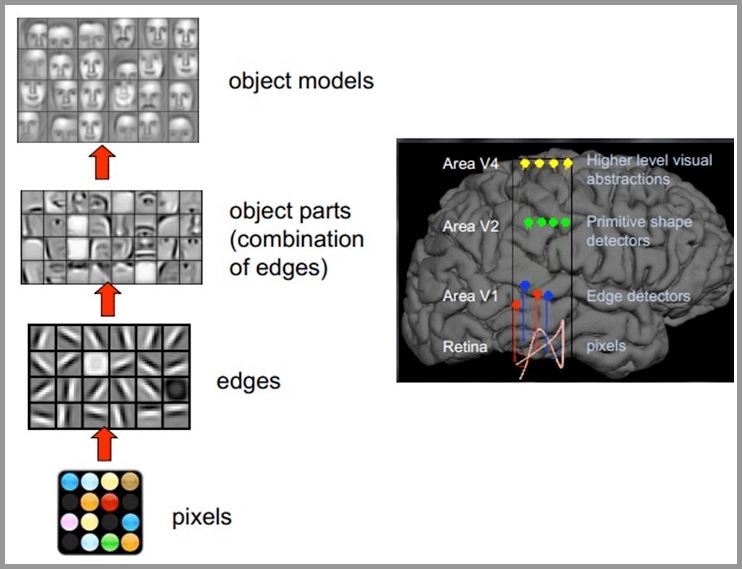
\includegraphics[height=5.5cm]{face_recognition.png}}
\caption{人脑识别人脸的过程示意图}
\end{figure}

对于不同的物体, 人类的视觉也是通过这样逐层分级来进行认知的: 
\begin{figure}[H]
\centering{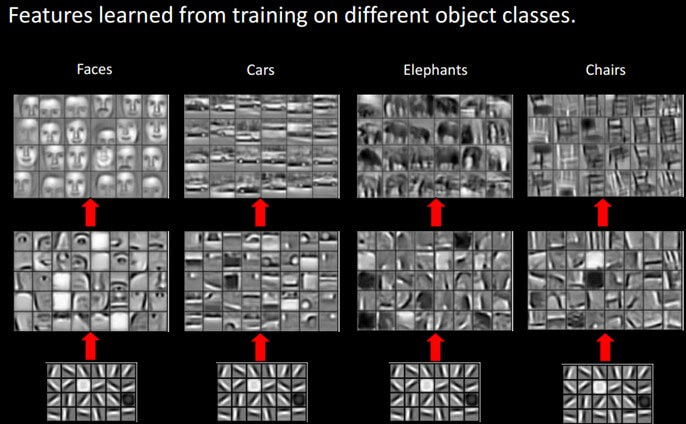
\includegraphics[height=5cm]{objects.jpg}}
\caption{人类对物体的逐层分级认知}
\end{figure}

我们可以看到, 各种不同的物体在最底层的特征基本上是类似的, 通常即为各种边缘. 在层级中越往上, 越能观察到此类物体的一些独有特征 (轮子, 眼睛, 躯干等). 到最上层, 不同的高级特征最终组合成相应的图像, 从而能够让人类准确的区分不同的物体. 

一个很自然的问题是, 可不可以模仿人类大脑的这个特点, 构造多层的神经网络, 利用较低层的识别初级的图像特征, 用若干底层特征组成更上一层的特征, 最终通过多个层级的组合, 在顶层做出分类? 这是许多深度学习算法, 包括卷积神经网络的灵感来源.

典型的卷积神经网络一般由三个部分构成:  卷积层, 池化层, 全连接层 \cite{khan18}. 如果用简单的语言进行描述, 卷积层主要会提取图像中的局部特征; 池化层主要用来降低参数量级 (降维); 全连接层类似传统神经网络的部分, 用来整合信息输出最后的结果. 

我们以图像处理为例详细介绍每一层的构成. 黑白图像的每一个像素块对应一个灰度值, 因此整张图像对应于一个非负的二维矩阵$M\in \mathbb{R}^{m\times n}$, 矩阵中元素的排列即为图像中像素块的排列. 传统的神经网络, 如MFN, 会将整个矩阵视作一个长向量$v\in \mathbb{R}^{mn}$. 然而, 这样的做法并没有充分的利用到图像不同像素块之间的位置信息, 并且若图像的分辨率很高, 构造神经网络的参数为非常多.

\subsubsection{卷积层}
卷积神经网络的卷积层的运算过程是以一个卷积核扫完整张图像 (矩阵$M$), 不同与传统神经网络的全连接并且以边权为参数, 卷积神经网络以卷积核的值为该层参数. 下图是用一个卷积核扫完整张图像的例子: 
\begin{figure}[H]
\centering{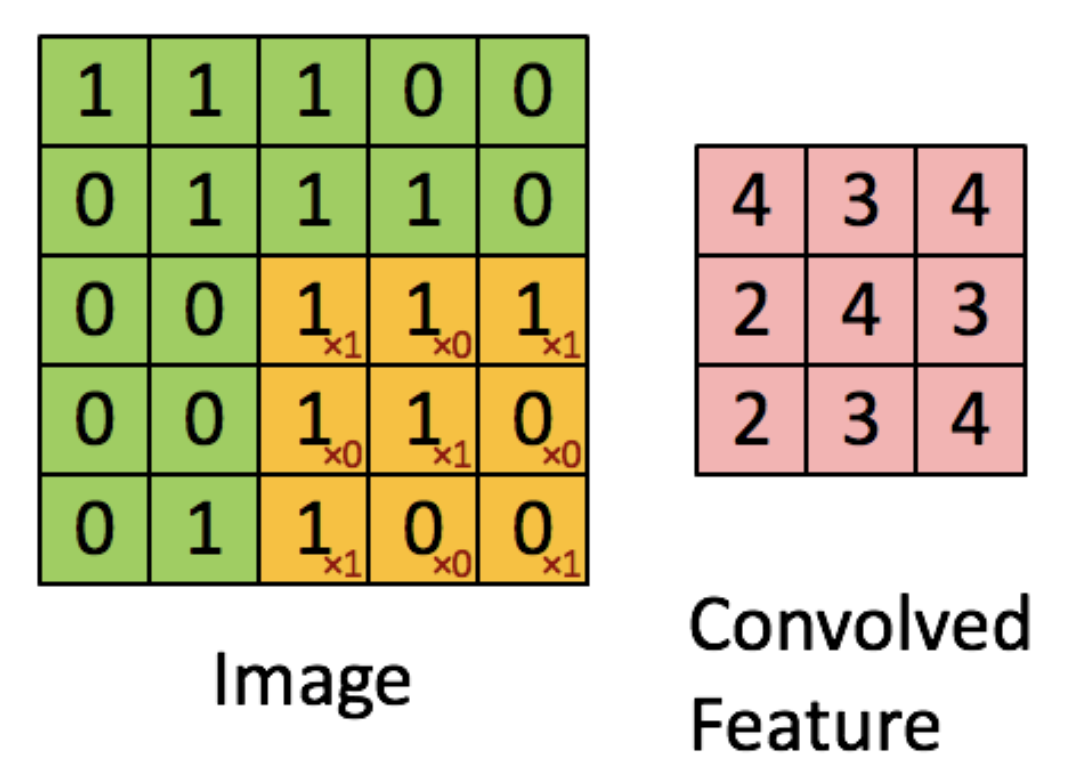
\includegraphics[height=5cm]{convolution.png}}
\caption{卷积层示意图}
\end{figure}

在该示意图中, 图像对应的是一个二维矩阵$M \in \mathbb{R}^{5\times 5}$, 我们采用了二维矩阵$\left (\begin{array}{lll}{1} & {1} & {1} \\ {1} & {1} & {0} \\ {1} & {0} & {0}\end{array}\right)$作为卷积核, 该卷积核以1为步长扫过整张图像. 图中的加深区域表示卷积核在该子区域上的作用, 该$3\times3$子矩阵的元素与卷积核的元素一一作用, 最后求和得到输出矩阵$\left (\begin{array}{lll}{4} & {3} & {4} \\ {2} & {4} & {3} \\ {2} & {3} & {4}\end{array}\right)$中的最后一个值, 4. 需要注意的一点是, 如全连接网络MFN一样, 我们不会仅仅采用这种通过线性组合得到的数据作为最终输出, 在这里同样需要引入激活函数. 通常, 我们仍需要选择合适的激活函数作用到输出矩阵中, 以作为下一层网络的输入.

我们可以抽象的理解卷积的过程, 我们用了一个向量$v \in \mathbb{R}^{25}$作为输入, 输出了另一个向量$u \in \mathbb{R}^{9}$. 但是我们并不采用$\mathbb{R}^{25}\rightarrow \mathbb{R}^{9}$的全连接, 一共引入$9\times 25 +1$个参数. 取而代之的, 我们只引入9个参数, 这9个参数重复的作为输入中的若干部分的权值. 在这个例子中, 我们采取了扫描步长为1, 如果选取步长为2, 那么卷积核在扫描的时候不再是每次平移一格, 而是平移两格, 对应的, 我们将得到一个$2\times 2$的输出矩阵. 通过这样的过程, 我们可以直观的感觉到, 如果能选择合适的卷积核, 我们不但可以降低维数 (减少参数的引入), 从而降低过拟合的风险, 也可以更好的利用图像中各像素块的位置信息. 我们可以将这个过程理解为使用一个过滤器 (卷积核) 来过滤图像的各个小区域, 从而得到这些小区域的特征. 

在真实的图像分类问题中, 我们遇到的通常是彩色图像, 其中每一个像素块都对应于RGB三个通道共三个值. 所以, 此时我们的输入不再是一个二维的矩阵, 有$M \in \mathbb{R}^{m\times n\times 3}$. 由于仍要考虑各个像素点的位置信息, 我们同样选择三维矩阵作为卷积核, 作用方式依旧为加权求和. 一个卷积核作用在输入图像上会得到一个二维的输出矩阵.

在具体应用中, 每一层往往有多个卷积核, 从而使输出的也是一个三维矩阵, 其第三个维度等于卷积核的数量. 可以认为, 每个卷积核代表了我们想要发现的一种图像模式, 如果某个图像块与此卷积核卷积出的值大, 则认为此图像块十分接近于此卷积核. 如果我们设计了6个卷积核, 可以理解成我们认为这个图像上有6种底层纹理模式, 即我们用这6种基础模式就能描绘出这幅图像. 以下是25种不同的卷积核提取出的特征的示例: 
\begin{figure}[H]
\centering{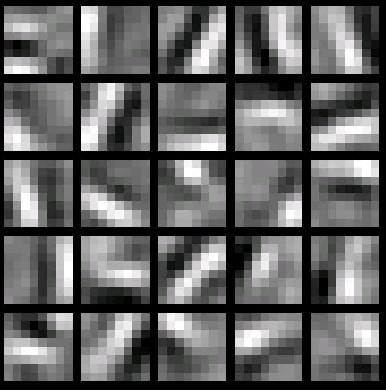
\includegraphics[height=5cm]{kernel.jpg}}
\caption{25种卷积核提取特征的示例}
\end{figure}

\subsubsection{池化层}
池化层简单说就是下采样, 可以通过该过程大大降低数据的维度. 在操作上, 池化层通常将输入的图像分块, 并从每一块中仅提取部分信息用以构成下一层的矩阵.
\begin{figure}[h]
\centering{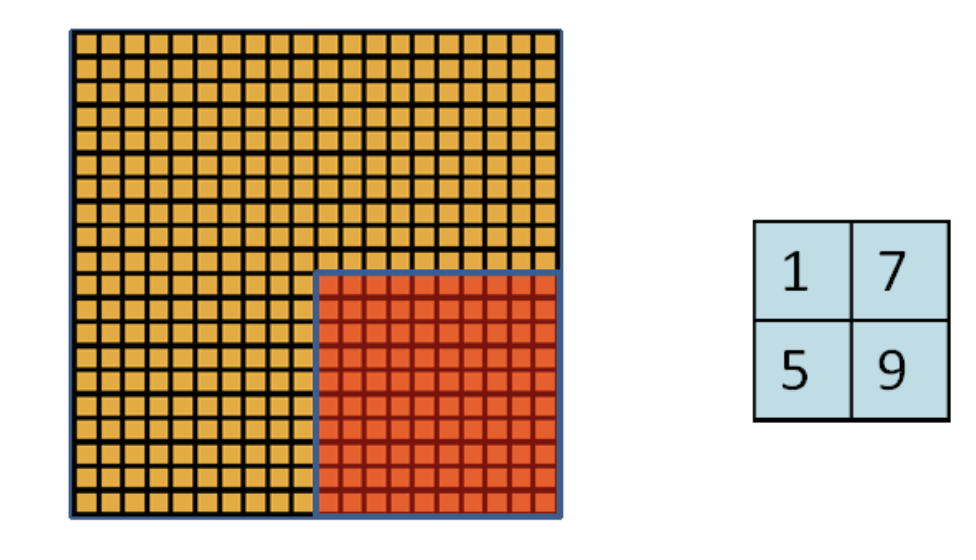
\includegraphics[height=4cm]{pooling.png}}
\caption{池化过程示意图}
\end{figure}

在池化层的示意图中, 我们可以看到原始图像对应一个$20\times20$的矩阵, 我们对其进行下采样, 采样窗口为$10\times10$, 最终得到一个$2\times2$大小的特征图. 常用的池化操作有:  提取最大值, 即提取示意图中红色区域矩阵的最大值作为输出矩阵相应位置的值 (图中为9); 求取平均值, 即求取目标区域中所有值的平均作为一个输出值. 在示意图中我们取了不相交区域分别进行池化, 实际应用中这不是必须的.

引入池化层的主要是因为即便做完了卷积, 数据的维度通常仍然很大, 这是因为我们为了提取特征, 常常使用维数较小的卷积核, 所以为了降低数据维度, 我们会进行这样的下采样操作. 这么做不但可以大大减少计算量, 还可以有效的避免过拟合.

\subsubsection{全连接层}
通常卷积神经网络以全连接层结束. 全连接层将之前乙烯类卷积层, 池化层共同输出的结果矩阵转化成一个长向量, 以图\ref{fig: fullconnection}的连接方式构造一个传统神经网络, 用于整合之前分层学到的信息, 以及输出最后的结果. 经过卷积层和池化层降维过的数据, 才能尽量保证我们不需要在全连接层中构造过于庞大的网络, 引入过多的参数. 

\subsection{完整的卷积神经网络及其训练}
典型的 CNN 通常并非只有以上介绍的3层结构, 而是这3种结构的有机组合形成的多层网络, 例如下图所示的 LeNet-5: 
\begin{figure}[H]
\label{fig: lenet}
\centering{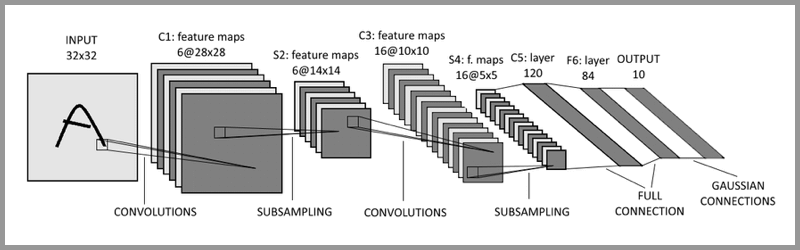
\includegraphics[height=4cm]{lenet.png}}
\caption{LeNet-5示意图}
\end{figure}
其结构大概是\textit{卷积层 – 池化层- 卷积层 – 池化层 – 卷积层 – 全连接层}, 其中第一个卷积层中引入了6个卷积核, 第二个卷积层中引入了16个卷积核.

关于 CNN 的训练, 需要注意我们想训练的参数是卷积核中的元素, 以及最后全连接层中的边权, 通常池化的方法都是人为给定的. 我们仍然可以像训练传统神经网络一样引入误差函数$E_{k}=\frac{1}{2} \sum_{j=1}^{l}\left (\hat{y}_{j}^{k}-y_{j}^{k}\right)^{2}$, 该误差函数是以网络中未知参数为变量的函数, 可以采用梯度下降法, 随机梯度下降法, 或者其他优化方法进行求解, 具体的推导方式我们在这里不详细给出.

\section{CNN模型具体探讨与理解}
图像的识别和分类的基本方法很多, 经过讨论, 我们认为CNN方法是最自然, 与课程联系最为紧密的一个方法.

为了解决CIFAR-100数据集的分类问题, 我们对神经网络进行了更深入的资料收集, 背景了解. 我们认为首先需要将注意力放在对图像的边缘检测上, 即检测边缘是图像识别的首要任务. 用这样的方法, 通过训练一定的给定图像集, 识别其水平与垂直的边缘, 可以较粗略地识别图像. 根据概率论课堂的知识, 我们认为利用过滤器 (filter) 和卷积来处理图像矩阵是最好的方法之一. 

我们选择利用卷积是因为处理较大的图像数据的时候, 我们可以更好地利用其参数共享 (parameter sharing) 和稀疏连接 (sparsity of connection) 的优势.  事实上, 我们认为特征检测, 如垂直边缘检测, 如果适用于图像的某个区域, 那么它也可能适用于图像的其他区域 (过滤器对于小方阵都是适用的, 所以节省了参数的选取). 我们设计了一些小型实验用于验证这个想法, 而实验证明当整张图像共用特征检测器, 提取效果甚至可能更好 (类似平移不变的性质), 这显示了卷积参数共享的性质. 稀疏连接的优势主要体现在一个输出单元仅与较少的参数提取相关, 而其他像素不会对输出产生影响. 因此可以用更小的训练集来进行训练, 降低了过度拟合的风险.
 
确定了大方向之后, 我们开始考虑如何具体进行计算求解并针对卷积神经网络的方法进行编译处理. 

\subsection{经典的CNN模型}
我们的讨论重点落实在了如何整合卷积上. 为此我们更深入地分析了一些既有的著名实例和一些经典网络如LeNet-5, AlexNet, VGGNet, ResNet, Inception网络等, 并研究这些网络中基本构件的组合方式 (注, 其中多种模型因深度过高, 我们省略其架构示意图).

其中, LeNet-5是1998年 Lecun 等人 \cite{lecun98} 提出的模型, 这个模型主要用于识别手写字符图像. 我们认为可以从这个经典模型上学到许多结构关系及具体的技巧. LeNet-5的各网络层之间是相互关联的, 并且采用了更多的最大池化的过程. 但是, 那时人们还未大量采用padding的手段来控制图像的大小, 当时Softmax输出采用了现在很少使用的输出层, 总共仅有约6万个参数, 远远低于现代版本的一千万至一亿个参数的规模. 此外, 人们最初使用的是Sigmoid函数和Tahn函数作为激活函数, 每个过滤器都采用和输入模块一样的信道数量, 这些都导致计算量过大, 代码过于复杂且繁琐, 我们认为不应在这次的任务中采用. 文献中提到的另一种思路“图形变形网络”如今还没有得到非常广泛的应用, 我们认为其有一定的阅读价值, 但并没有在本次任务中采用. 

AlexNet是另一种非常适宜用于计算机视觉任务的模型, 由 Krizhevsky 等人 \cite{krizhevsky12} 在2012年提出. 最初的AlexNet包含了6000万个参数, 相当复杂. 但是当用于训练图像数据集时, AlexNet往往能够处理非常相似的基本构造模块, 这些模块中往往包含大量的隐藏单元或数据. 不过这篇论文发表的时候, GPU的处理速度还比较慢, 因此AlexNet采用了非常复杂的方法在2个GPU上进行训练, 也就是将这些层分拆到2个不同的GPU上, 同时建立一个方法用于2个GPU之间进行交流, 这一点在目前是不必要的, 因此我们可以大大简化. 此外, 在AlexNet中引入了一种"局部相应归一化层" (LRN层), 这类层的应用不是非常广泛, 它指的是选取一个位置, 从这个位置穿过整个信道, 实现归一化, 从而我们可能并不需要太多的高激活神经元. 但LRN在实际的应用当中并没有起到预想中的作用, 因此我们认为不需要用LRN来训练网络. 
\begin{figure}[H]
\label{fig: lenet}
\centering{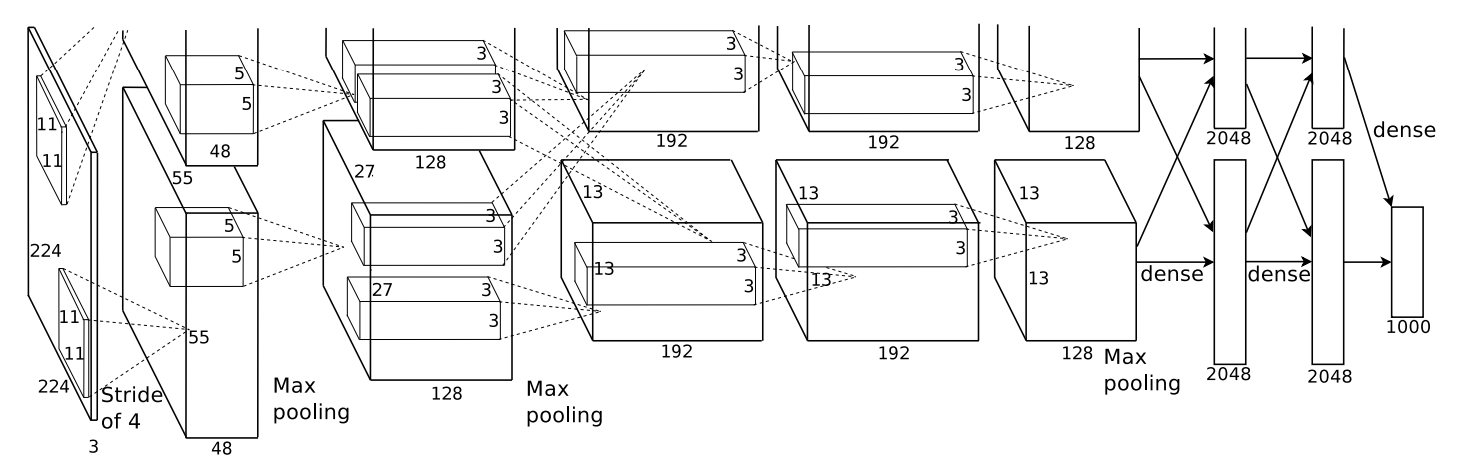
\includegraphics[height=5cm]{alexnet.png}}
\caption{AlexNet架构示意图}
\end{figure}

VGG-16则是一种专注于构建卷积的简单网络, 由 Simonyan 等人 \cite{simonyan14} 在2014年提出. VGG-16通过padding和构建最大池化层的方法, 建立了简单的神经网络结构. 接着, 池化层将图像进行压缩, 最终经过全连接层, 用Softmax激活. VGG-16有16个卷积-池化层, 有1.38亿个参数, 是一个很大的网络, 但是它的结构非常简单和规整. 我们最感兴趣的是, 在论文中指出, 随着网络的加深, 图像的高度和宽度都在以一定的规律不断缩小, 每次池化后刚好缩小一半, 而信道数在不断增加, 并且恰好在每组卷积操作后增加一倍, 也就是说图像缩小的比例和信道增加的比例是有规律的. 这个网络带给我们的启示是, 一个或者多个卷积层后面跟着一个池化层的排列方式是常用且有效的. 

He 等人 \cite{he16} 在2016年提出了ResNet. 它是由残差块组成的, 利用远跳连接构建的深度训练网络, 深度高达100. 残差块在进行线性激活后, 乘以权重矩阵, 加上偏差因子, 再多次重复ReLu非线性激活与线性激活的过程. 这构成了网络层的主路径.  ResNet就是大量的残差块堆积在一起构成的神经网络. ResNet带给我们的启示是在当我们需要进一步提高神经网络的训练深度的时候, 可以借鉴运用残差块的方法来处理问题. 我们在实验中发现的一个问题可以被ResNet引入残差块的想法较好的解决:  在理论上, 网络深度通常与预测正确率正相关, 然而在真实实验中, 由于过拟合现象, 训练错误常随着网络的加深先减后增. 而对于ResNet, 它的预测错误率并不随训练深度增加而增加, 这种表现引起了我们的讨论和深思. 

Szegedy 等人 \cite{szegedy15} 在2015年提出了 Inception 网络, 该网络可以"智能"的确定是否需要创建卷积层, 使用哪个过滤器, 或者是否需要池化, 免去了人工判断的需要.  然而相应的, 需要计算输出的计算成本会有一定的增加. 解决方法通常是先缩小网络表示再扩大它, 但是相比其他网络, 此时的计算成本仍然较高, 不适宜应用于本次大作业中的处理. 

综上所述, 如同课堂中所提到的, 卷积神经网络能很好地解决这样的类似问题, 而不同的卷积核的引入会得到不同的结果. 在具体的代码编写过程当中, 我们发现为了提升分类效率, 适当地选择filter以及其他重要的参数成为了一个重要的问题. 另一个基本问题是, 如何在算法中更优化地处理矩阵以及如何具体地对CNN中的每个层中的数据进行解释和编译. 基于这些基本的资料查找, 以及对于CNN的基本了解, 我们开始着手代码编写. 下面则是我们的具体的编译过程的思考与总结. 

\subsection{代码编译过程的理解与反思}
\subsubsection{卷积层的进一步理解}
卷积层的主要计算即卷积运算. 在Python中, 常常是通过Conv-forward来实现. 为了防止图像在每一次做了卷积运算之后缩小, 我们认为有必要采用padding的技巧, 即在图像的四周增加值为0的空像素. 另一方面, 为了能够顺利地拟合, 我们需要采用规模为奇数的过滤器, 并且在计算经过padding的图像的时候取Gauss函数来保证它的规模是一个整数.
 
此时再考虑RGB图像的情况, 它是三个图层 (红色, 绿色, 蓝色的三色复合得到一般的图像)复合的结果. 选取$n_c$个filter, 再增加偏差, 应用非线性函数复合 (一般地, 是ReLu非线性函数), 最终得到输出项. 这里选取多个filter是为了避免过拟合. 总而言之, 我们认为可以利用Python的广播机制, 给所有的矩阵中的元素 (此处的矩阵指的是进行了卷积变换的矩阵)都加上同一个偏差值, 再复合上ReLu的非线性激活函数. 

Filter的选取也取决于我们的目的. 如果是要考察一个特定颜色的边缘, 如R的横向边缘, 我们认为即将R对应的filter取值为常用取值, 而G, B的filter则取为0矩阵, 再把它们堆叠起来, 就可以得到结果. 而如果不是考虑特定颜色的横向边缘, 我们仅需要考察3个filter都取值为常用取值得到的结果. 纵向边缘同理. 

综上所述, 在卷积层中, 我们设想的基本操作是在必要的时候采用padding和stride (调整步长)的方法, 每次将原矩阵与filter进行卷积运算. 这时候需要选定的待定参数有filter的规模大小f, padding的选取大小p, 调整步长的取值s, 在一些特别的情形下, p, s都可以取值为0.

为此我们首先研究了ConvNet的卷积层在维数较低的情形下的计算, 再针对实验数据的卷积层进一步处理. 

\subsubsection{池化层和全连接层的进一步理解}
我们认为有必要在方法中建立一些池化层, 来减小模型大小, 提高效率. 我们根据文献中的材料得知, 池化过程应用的最广泛的技巧是最大池化方法: 即拆分矩阵为一些更小的方阵, 选取其中每个方阵中的最大值. 一般地, 采用最大池化的常用参数 (hyper parameters of max pooling)使用一个规模为f的filter, 采用步幅为s的卷积算法. 这时得到的矩阵可以视为某些特征的集合. 

这一组参数 (hyper parameters of max pooling)的存在并没有导致我们需要学习参数, 实际上, 我们可以较直观地看到, 梯度下降运算在确定了f (filter规模)和s (步幅)之后就是一个固定的运算, 无需改变任何值. 

因此根据文献的查找以及对于更小的图像的具体实践, 我们认为池化层的添加确实可以提高效率. 我们还了解到, 除了最大池化法, 常用的池化法还有平均池化的方法, 但是在粗糙的识别代码运行下, 我们依然更倾向于采用最大池化的方法. 

由于我们需要处理一般的图像识别的情况, 因此我们考虑对于高维信道的情形, 单独执行最大池化法. 在这个过程中, 我们需要考察隐藏层, 而一般的全连接层是一个标准的神经网络, 与我们在课堂中所学到的神经网络有更大的似合性. 它是具有一个权重矩阵, 具有偏差参数, 因此我们依照在概率论研讨课中所学习的知识对它进行了编译, 最终仅需再考虑softmax的输出 (根据分类的粗细可以定出具体的输出数值)即可. 

\subsubsection{卷积神经网络的构建}
在参考了上文所述经典的神经网络之后, 我们了解了最简单的神经网络的搭建, 因此经过卷积运算, 将第一个卷积层命名为Conv1, 之后采取的第一个池化层命名为Pool1, 我们认为它们构成了神经网络的第一层 (因为池化层没有权重和参数, 一般与卷积层合并称为一层)得到Layer1. 

同理, 为了提升训练的深度, 我们达成再搭建N个Layer的共识, 并将LayerN平整化后得到一维向量, 我们将它视为一个神经元集合. 最终, 我们利用这些单元构建下一层, 得到全连接层, 并通过激活输出.
 
在具体的研究过程中, 需要注意的是随着神经网络深度增加, 矩阵的行列 (对应图像的长度, 宽度)都会减少, 而信道数量 (层数)会增加. 我们发现, 激活值会随着过程降低, 这与一般的神经网络的基本结构是一致的. 在尝试的过程中, 我们也采取过多个卷积层后接着一个池化层的结构. 

\section{层级深度卷积神经网络 (HD-CNN)}
在图像分类任务中, 不同类别之间的视觉可分离性非常不均匀, 即某些类别比其他类别更难区分. 以我们本次的分类任务的数据集CIFAR-100为例, 这些图像共有20个粗糙类别与100个精细的类别, 相对分类处于不同粗糙类别中的图像, 如苹果与公交车, 可以想见的是更难区分处于同一粗糙类别中的图像, 如苹果与橘子 (这两者都属于水果大类, 而公交车属于汽车大类). 对于如图\ref{fig: lenet}所示的基本的卷积神经网络, 其输出神经元是位于同层的并列神经元, 这使得其并不那么容易剥离数据中的层级信息, 区分粗糙类与精细类. 这样的困难暗示我们可能需要引入一些专门的操作.

我们发现 Yan 等人 \cite{yan15} 于2014年提出的层级深度卷积神经网络的模型 (Hierarchical Deep Convolutional Neural Network, HD-CNN) 能够更好地处理类似这样的问题. 该网络的特别之处是, 他可以基于任一普通的卷积神经网络 (如图\ref{fig: fullconnection}) 进行构建, 引入分层的分类模式, 进而进一步提高基层CNN对不均匀分类的准确性. 因此, 如果采用本身准确率就比较高的CNN作为基层网络, 进行层级化处理后, 能得到准确率更高的网络. 
\subsection{HD-CNN的架构}
HD-CNN的架构示意图如下.
\begin{figure}[H]
\label{fig: hdcnn}
\centering{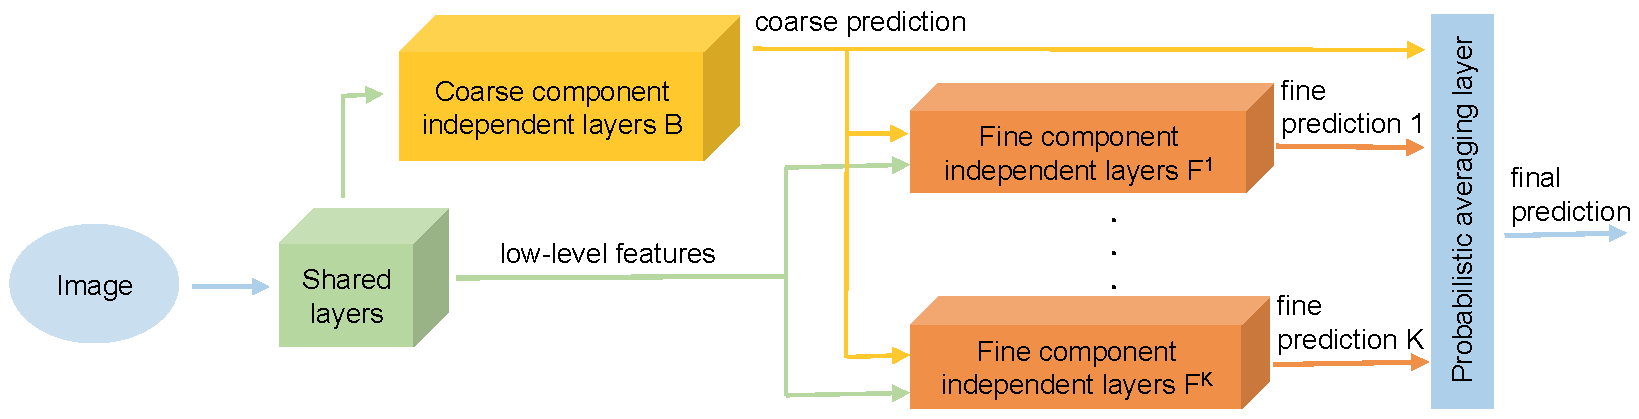
\includegraphics[height=3.5cm]{hd-cnn.png}}
\caption{HD-CNN架构示意图}
\end{figure}

从图中可以看到, HD-CNN主要有四个部分组成, 分别是共用层, 单个粗糙分类器$B$, 多个精细分类器$\left\{F^{k}\right\}_{k=1}^{K}$, 以及概率平均层 (决定输出). 我们逐步介绍HD-CNN各部分的作用, 以及原理.

\begin{enumerate}
	\item 共用层的作用主要是接受输入的图像 (不妨表示为$\left\{\mathbf{x}_{i}, y_{i}\right\}_{i}$, 其中$y_i$是标记), 并且从中提取低级的特征, 如图像的边, 角等. 这些基本信息对于粗糙分类与精细分类都有用处, 因此该层是共用的 (并且共用还有降低计算量, 减少参数的好处). 在实际操作中, 我们选取基层CNN的浅层部分作为HD-CNN的共用层.
	\item 架构示意图的左上部是用于粗分类的组件. 这部分的网络重新利用了基层CNN的深层部分 (后端). 通过基层CNN, 我们可以生成一个图像的精细分类, 而该部分组件利用这个初步生成的精细分类, 做进一步的精细到粗糙的聚集过程, 即给出一个映射$P: [1, C] \mapsto[1, K]$, 其中$[1, C]$对应精细类别$\left\{S_{j}^{f}\right\}_{j=1}^{C}$, $[1, K]$对应粗糙类别$\left\{S_{k}^{c}\right\}_{k=1}^{K}$. 事实上, 粗分类组件将会输出若干概率值, 用于表示该图像属于某一分类的后验概率.
	\item 右下部分是一些独立的精细分类器, 用于细分通过之前操作得到的粗糙分类$\left\{F^{k}\right\}_{k=1}^{K}$. 这部分的组件通常也由基层CNN中的子网络直接构成, 只需要对输出层进行一定调整.
	\item 架构示意图的最右部分是概率平均层, 将以粗糙层输出的后验概率为权重, 对精细层输出的预测进行加权平均. 最终的预测结果为 $p\left (\mathbf{x}_{i}\right)=\frac{\sum_{k=1}^{K} B_{i k} p_{k}\left (\mathbf{x}_{i}\right)}{\sum_{k=1}^{K} B_{i k}}$, 其中$B_{i k}$是$\mathbf{x}_i$在粗糙分类器$B$的预测下属于第$k$粗糙类的概率, $p_{k}\left (\mathbf{x}_{i}\right)$是精细分类器$F^k$输出的预测值.
\end{enumerate}

\subsection{学习类别层次结构}
构建HD-CNN的时候, 构建类别层次结构是通过将容易混淆的精细分类归为同一粗糙分类, 然后再训练专用精细分类器完成的.

首先, 我们将从训练集中随机抽取一部分的样本, 并将剩余的样本用于训练基层CNN. 对于抽取的样本, 我们将构建一个混淆矩阵$\mathbf{F}$, 以及对应的距离矩阵$\mathbf{D}=1-\mathbf{F}$, 不妨设其是对称的 (否则可以对称化, $\mathbf{D}=0.5 *\left (\mathbf{D}+\mathbf{D}^{T}\right)$). 距离矩阵的元素$\mathbf{D}_{i j}$衡量区分类别$i$与类别$j$的难易程度, 即该数越大则越容易区分. 通过研究矩阵$\mathbf{D}$, 我们可以得到一个初步的分类映射$P^{d}: [1, C] \mapsto[1, K]$, 其中不同粗糙类别包含的精细类别不相交.

然而这样做略有偏颇, 因为后续的精细分类器不会只在粗糙分类中进行细分类的操作, 若一个图像对应的粗糙分类错误, 这个错误并不能被纠正, 从而整体的分类成功率十分依赖于映射$P^{d}$. 因此, 我们选择将一些精细类别加入多个粗糙类别中, 即构造一个集合到集合的函数$P^{o}: [1, C] \mapsto[1, K]$. 具体操作上, 设$F^k$是一个精细分类器, 我们按照下式估计把一副属于精细类别$j$的图像错误分类到粗糙类别$k$的似然: 
\begin{equation}
u^{k} (j)=\frac{1}{\left|S_{j}^{f}\right|} \sum_{i \in S_{j}^{f}} B_{i k}^{d}
\end{equation}
其中, 与之前相同, 下标中的$i$代表图像$\mathbf{x}_i$, $B_{i k}^{d}$是根据$P^d$聚集精细类别概率$\left\{B_{i j}^{f}\right\}_{j}$得到的粗糙类别$k$的对应概率, 即$B_{i k}^{d}=\sum_{j | P^{d} (j)=k} B_{i j}^{f}$. 我们设置一个阈值, 例如$u_{t}= (\gamma K)^{-1}$, 将那些满足$u^{k} (j) \geq u_{t}$的精细类别$j$都加入到粗糙类$S_{k}^{c}$中, 这样我们就得到了一个集合间的映射$P^o$. 特别, 如果设置$u_t = 0$, 则任一粗糙类别均包含了所有精细类别, 如果$u_t = 1$, 则$P^o = P^d$.

\subsection{HD-CNN的训练}
当我们将精细分类组件嵌入到HD-CNN中时, 后层的参数数量将随着粗糙类别的数量线性增长. 在相同数量的训练图像的情况下, 这会增加训练的复杂性和过度拟合的风险. 另一方面, 在采用随机梯度下降法时mini-batch的大小也需要随着参数增加而上升, 这会增加内存占用量并减慢训练过程. 因此, 我们需要将HD-CNN的训练分解为多个步骤, 而不是简单的从头开始按顺序训练.

我们依次对粗糙分类和精细分类进行预训练. 首先注意到, 由于粗糙分类组件主要基于基层CNN的结构与输出构建, 我们可以将训练基层CNN$F^{p}$得到的参数作为该组件的初始化参数. 对于精细分类组件$\left\{F^{k}\right\}_{k}$, 我们可以并行的进行预训练, 每一个组件$F^k$只需要专门在相应的粗糙类别$S_{k}^{c}$中激进型训练, 其初始化参数依旧可以沿用基层CNN $F^p$的参数.

在结束粗糙分类组件和精细分类组件的预训练后, 我们对整个HD-CNN进行微调. 注意到, 在类别层次结构确定后, 每个精细分类组件支仅专注于分类某一特定子类别. 我们在微调过程中, 需要保持由粗糙分类器给出的粗糙类别与后续精细分类器所分的精细类别所处粗糙类的一致性. 以下, 我们设计一个损失函数中罚项来保证这一点.

学习得到的精细-粗糙映射$P: [1, C] \mapsto[1, K]$给我们提供了一个表示粗糙分类分布$\left\{t_{k}\right\}$的方式. 特别, $t_{k}$是那些``可能''被映射分到粗糙类别$k$的图像的比重, 即
\begin{equation}
t_{k}=\frac{\sum_{j | k \in P (j)}\left|S_{j}\right|}{\sum_{k^{\prime}=1}^{K} \sum_{j | k^{\prime} \in P (j)}\left|S_{j}\right|} \quad \forall k \in[1, K]
\end{equation}

从而, 我们可以决定损失函数: 
\begin{equation}
E=-\frac{1}{n} \sum_{i=1}^{n} \log \left (p_{y_{i}}\right)+\frac{\lambda}{2} \sum_{k=1}^{K}\left (t_{k}-\frac{1}{n} \sum_{i=1}^{n} B_{i k}\right)^{2}
\end{equation}
其中, 第一项是对应于分类正确率的罚项, 第二项对应以上我们想要保证的一致性.


\section{K-近邻算法 (KNN)}
除了CNN方法外, 我们组同时也考虑了使用KNN算法实现图像分类的,作为对主体算法的有力补充.

K-近邻算法 (KNN)是最基本的一种机器学习方法. 在本次实验中,  我们尝试使用KNN进行图像分类的任务, 考察KNN的学习效果并思考相关改进方法.其具体代码见附录.
%,  同时与我们最终确定的卷积神经网络方法进行对比,  比较两种方法的优劣
\subsection{KNN算法简介}
在KNN方法中,  首先假定所有的实例对应n维空间$R^{n}$中的点,  即对任意实例$x$,  将其表示为一个特征向量$<a_{1} (x), a_{2} (x), ..., a_{n} (x)>$,  其中$a_{i} (x)$对应实例的第$i$个属性值. 实例的最近邻由标准欧氏距离$d (x_{i}, x_{j}) = \sqrt{\sum_{r=1}^{n}{ (a_{r} (x_{i})-a_{r} (x_{j}))^{2}}}$定义. 

以学习离散目标函数$f:  R^{n} \rightarrow V$过程为例简述KNN算法思路. 在训练算法中,  将每个训练样例$<x,  f (x)>$加入到列表training-example中. 在分类算法中,  给定查询实例$x_{q}$,  首先在training-example中选出最靠近$x_{q}$的k个实例,  记为$x{i}, i=1,  2,  ...k$. 以这$k$个实例中最普遍的实例所在的样例作为$x_{q}$的分类,  即$ \hat f (x_{q}) \leftarrow argmax{\sum_{i=1}^{k} \delta (v,  f (x_{i}))}$. 若a不等于b,  $\delta (a,  b)=0$,  否则为1. 对于连续值目标函数,  将公式替换为$\hat f (x_{q}) \leftarrow \frac{\sum_{i=1}^{k}{f (x_{i})}}{k}$. 

\subsection{实验结果分析}
实验结果如下表所示,  对“粗糙标签”的分类,  KNN的准确率在$24\%$到$27\%$之间,  对“精细标签”的分类,  KNN的准确率在$14\%$到$18\% $之间. 在实现分类任务的同时,  通过尝试不同的K寻找最优值. 受限于时间和计算机性能,  只测试了K为1,  2,  3,  4,  5这五个值,  发现$K=1$时在本次分类实验中取得最优效果. 
\begin{table}[htbp]
\centering
\begin{tabular}{|c|c|c|c|c|c|}% 通过添加 | 来表示是否需要绘制竖线
	\hline  % 在表格最上方绘制横线
	K&1&2&3&4&5\\
	\hline  %在第一行和第二行之间绘制横线
	{准确率 (粗糙标签)}&0.2641&0.2411&0.2401&0.2481&0.2476\\
	\hline % 在表格最下方绘制横线
	{准确率 (精细标签)}&0.1754&0.1491&0.1479&0.1498&0.1504\\
	\hline
\end{tabular}
\caption{KNN初步测试结果}
\end{table}
从实验结果中发现,  面对较为庞大的数据集时,  KNN的分类准确率不甚理想. 在运算速度上,  由于KNN分类时需要对所有样例进行距离计算,  因此计算量也比较大,  收敛速度不快. 这导致通过逐一测试寻找最优k值的方法在大样本情形下不适用. 

\subsection{KNN算法优化}
在本节中, 我们介绍几种从提高精度, 提高运算速度和寻找最优K值的角度对KNN进行优化的方法.
\subsubsection{距离加权最近邻算法\cite{Mitchell97}}
在该算法中,  我们通过对k个近邻的贡献加权,  即根据他们相对查询点$x_{q}$的距离,  将较大的权重赋给较近的近邻. 对离散情形,  修改后的公式为$ \hat f (x_{q}) \leftarrow argmax{\sum_{i=1}^{k} {w_{i}}\delta (v,  f (x_{i}))}$,  其中,  $w_{i}$是良定义的权重函数. 类似的,  对连续情形公式修改为${\hat f (x_{q}) \leftarrow \frac{\sum_{i=1}^{k}{w_{i}f (x_{i})}}{\sum_{i=1}^{k}{w_{i}}}}$. 在实验中,  选取权重函数$w_{i} (x_{i},  x_{j}) = d (x_{i},  x_{j})$,  加权后得到如下结果: 
\begin{table}[htbp]
\centering
\begin{tabular}{|c|c|c|}% 通过添加 | 来表示是否需要绘制竖线
	\hline  % 在表格最上方绘制横线
	K&2&3\\
	\hline  %在第一行和第二行之间绘制横线
	{准确率 (粗糙标签)}&0.2641&0.2636\\
	\hline % 在表格最下方绘制横线
	{准确率 (精细标签)}&0.1755&0.1753\\
	\hline
\end{tabular}
\caption{距离加权最邻近算法实验结果}
\end{table}
由此可以看出,  通过加权处理,  KNN算法能够有效处理训练数据中的噪声,  算法准确率得到提高. 

\subsubsection{QKNN (快速K-近邻算法)}
KNN算法的效率主要受制于样本量及样例空间维度. 由于对每个测试点的分类都要计算该点与所有样例的距离并排序,  而距离计算的运算量又随维度增加而提高,  因此对大样本, 特征复杂的分类任务KNN的运算效率较低. 

Chen 等人 \cite{chen18} 提出了一种QKNN的思路,  不去直接计算待测点$x$与所有样例$y_{i}$的距离,  而是先在样例$y_{i}$中选取一个参考点R,  将样例按照到参考点的距离$d (y_{i},  R)$进行排序,  构造一个有序训练空间. 之后计算待测点到基本点的距离$d_{xR}$. 在有序训练空间中寻找最接近$d_{xR}$的$d (y_{i},  R)$对应的样例q,  以q为中心确定其前后共k个点作为第一代k近邻,  之后按照一定规则从第一代k近邻出发向前, 向后搜索距离待测点更近的样例并更新k近邻. 按照该方法,  在分类时不再需要对所有的待测点与样本点的距离$d (y_{i},  x)$进行排序,  因此减少了运算量,  提高运算效率. 

\subsubsection{动态K-近邻算法}
KNN方法中最优的k的确定方法通常是逐一计算比较,  之后确定一个固定的值. 但在实际分类问题中,  不同的类可能对应不同规模的数据,  k选为定值可能会带来偏差. 例如对规模较大的类,  由于本身数据较多,  其中样例出现在某个测试点的k近邻中概率也会相应增大. 解决这一问题的想法是采用一个动态的依赖于类的大小的k. 以采用公式$${y (d_{i}) = argmax_{k} \sum_{x_{j} \in kNN}{Sim (d_{i},  x{j}) \delta (x_{j},  c_{k})}}$$的KNN算法为例 \cite{chen18} 分析动态算法 ($d_{i}$为待测点,  $x_{j}$为k个近邻点,  Sim为权重函数),  具体过程如下: 
\begin{enumerate}
	\item 按照一般KNN方法获得最初的k个近邻;
	\item 对一个类$c_{m}$,  在k个近邻$x_{1},  x_{2},  ...x_{m}$中选取n个最靠近$c_{m}$的样例$x_{i1},  ...,  x_{in}$,  其中n的选取取决于类$c_{m}$的规模;
	\item 修改公式为$y (d_{i}) = argmax_{m} \frac{\sum_{x_{j} \in n-kNN (c_{m})}{Sim (d_{i},  x{j}) \delta (x_{j},  c_{k})}}{\sum_{x_{j} \in n-kNN (c_{m})Sim (d_{i},  x_{j})}}$. 这里$n-kNN (c_{m})$代表每个类$c_{m}$对应的n个近邻的集合.
\end{enumerate}

\subsection{KNN小结}
本篇报告记录了使用KNN算法实现CIFAR-100分类的实验过程, 结果,  对于KNN算法在具体应用中出现的准确率低, 运算时间长进行了进一步的调研, 并利用距离加权最近邻方法实现了优化分类. 但对于QKNN以及动态k方法, 尚未进行代码实现, 因此这两种方法在CIFAR-100分类中的优化效果缺乏实验检验, 是下一步实验的一个方向. 


\nocite{*}
\bibliography{wpref}

\section*{附录: 分工安排}
\begin{itemize}
	\item 韩菲雨: 经典CNN模型的总结与改进, 对CNN算法及其代码调研 (与孙行之, 应东昊合作), 代码编译过程的反思与理解, 报告整理总结 (与应东昊合作).
	\item 林津伊: 朴素贝叶斯, 迁移模型, BP神经网络的调研与总结, 学习多种分类算法.
	\item 孙睿: KNN方法的调研总结与改进, 用KNN方法及Python环境实现图像分类的代码.
	\item 孙行之: 对CNN算法及其代码调研 (与应东昊, 韩菲雨合作), 用CNN方法及Python环境实现图像分类的代码, 代码汇总与管理.
	\item 谢沁昕: SVM方法的调研总结与改进.
	\item 应东昊: 前馈神经网络与卷积神经网络的调研与总结, HD-CNN的调研总结与改进, 对CNN算法及其代码调研 (与孙行之, 韩菲雨合作), 报告整理总结 (与韩菲雨合作).
\end{itemize}


\end{document}
